\chapter{Wissenschaftliche Grundlagen}
\section{Planare Graphen}
Zur einfacheren Handhabung des Grundrisses wird dieser in einen planaren Graphen umgewandelt. 
Ein planarer, auch plättbarer Graph ist ein Graph der in einer Ebene mithilfe von Punkten bzw. Knoten und Kanten dargestellt werden kann, ohne dass sich zwei oder mehr Kanten schneiden (vgl. Quelle \cite{planarGraph}). 
Jede Fläche des Graphen wird dabei durch mindestens drei verschiedene Kanten beschrieben, die den Rand dieser Fläche darstellen. 
Die Fläche um den Graphen herum, welche scheinbar unbegrenzt groß ist, wird äußeres Gebiet genannt.
\begin{Bild}{Schema eines planaren Graphen (Abbildung der Verfasser)}
	
\includegraphics[width = 100px, height = 100px]{Bilder/Graph_Scheme}
\end{Bild}
In Abbildung~\thebildnr\ wird ein solcher planarer Graph dargestellt.
Der linke obere Knoten wir hier mit (1) bezeichnet, die rechte Kante mit (2) und die innere Fläche mit (3).

\section{Doubly connected edge list}
Um planare Graphen ohne Informationsverlust zu speichern werden in der Informatik Referenzen zwischen den einzelnen Bestandteilen des Graphen eingesetzt. \\
In der sogenannten \q{Doubly connected edge list} (DCEL) erhält eine Kante, die aus einem Anfangsknoten und Endknoten besteht, jeweils eine Vorgänger-, eine Nachfolger- und eine Zwillingskante. 
Die jeweiligen Zwillingskanten beschreiben hierbei die invertierten Varianten der betrachteten Kanten.
Jedem Knoten wird außerdem eine ausgehende Kante und allen Flächen eine anliegende Kante zugewiesen (vgl. Quelle \cite{dcel} und \cite{dcelwiki}). \\
\begin{Bild}{Schema einer DCEL (Abbildung der Verfasser)}
	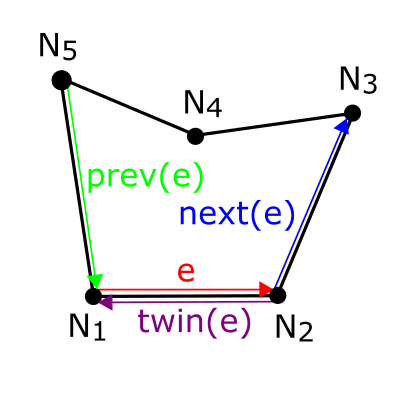
\includegraphics[width=150px]{Bilder/DCEL_Scheme}
\end{Bild}
In Abbildung~\thebildnr\ wird die Kante \q{e} durch den Anfangsknoten durch \q{N\textsubscript{1}} und den Endknoten \q{N\textsubscript{2}} gebildet.
Die Zwillingskante wird mit \q{twin(e)} bezeichnet, die Nachfolgerkante mit \q{next(e)} und die Vorgängerkante mit \q{prev(e)}. \\
Diese Referenzierungen ermöglichen es, ausgehend von einem Element ohne umfangreiche Berechnungen auf alle anderen Objekte zu schließen, indem bei der Betrachtung von Knoten und Flächen die zugehörigen Kanten, beziehungsweise bei der Betrachtung von einzelnen Kanten deren Vorgänger und Nachfolger betrachtet werden.

\todoinline{Johann wollte DCEL noch mal überarbeiten}

\section{AutoCAD}
%Konstruktionsprogramm statt architektenprogramm
AutoCAD ist ein grafischer Zeichnungseditor, welcher zum Erstellen von technischen Zeichnungen und dem Modellieren von Objekten verwendet wird (siehe Quelle \cite{autocadwiki}).
AutoCAD verwendet dabei einfache Objekte wie Linien, Kreise und Bögen, um auf deren Grundlage kompliziertere Objekte zu erschaffen.
Zu AutoCAD gehörig wurde das Dateiformat \q{.dxf} entwickelt, welches als Industriestandard zum Austausch von CAD-Dateien dient. \\
\begin{Bild}{Grundriss aus AutoCAD (Screenshot der Verfasser)}
	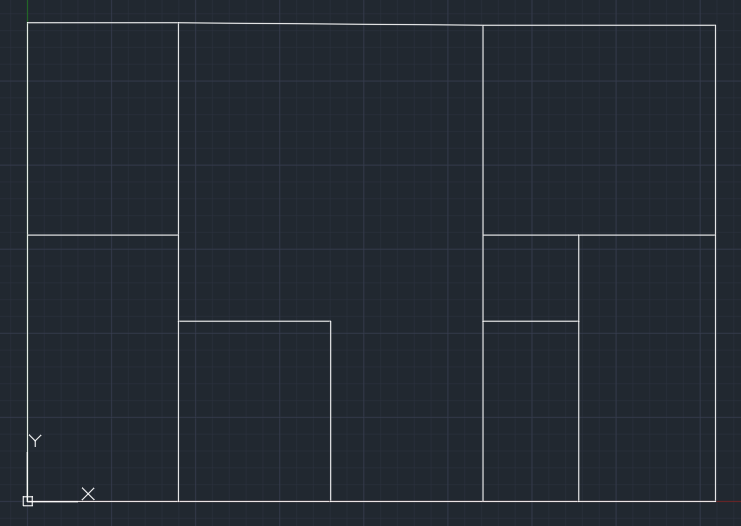
\includegraphics[width=\textwidth]{Bilder/Grundriss}
\end{Bild}
Der Grundriss, welcher als Ausgangspunkt dieser Arbeit fungiert, wird in AutoCAD erstellt und dem zu erstellenden Programm in Form einer .dxf-Datei bereitgestellt.
Diese Dateien dienen auch dem fertiggestellten Programm als Ausgangspunkt.
Ein Beispiel für einen solchen Grundriss ist in Abbildung~\thebildnr\ zu sehen.

\section{OpenSCAD}
OpenSCAD ist eine kostenlos verfügbare CAD-Modellierungssoftware, welche aus einer textbasierten Beschreibungssprache 3D-Modelle erzeugt (siehe Quelle \cite{OpenScad}).
OpenSCAD bietet dabei verschiedene Vorteile während des Modellierungsvorganges.
Hierzu gehören beispielsweise das farbige Hervorheben oder die Modularisierung zusammenhängender Objekte. \\
%Modellierung
Die Modellierung von einfachen Basisobjekten in OpenSCAD erfolgt durch das Verwenden von Schlüsselwörtern wie \icode{cube()}, \icode{sphere()} oder \icode{cylinder()} und Parametern in Klammern.
Diese Basisobjekte können anschließend durch Mengenoperationen wie Vereinigungen (\icode{union()}), Differenzen (\icode{difference()}) oder Überschneidungen (\icode{intersection()}) und Transformationen wie Skalierungen (\icode{scale()}), Rotationen (\icode{rotate()}) oder Translationen (\icode{translate()}) mit einander verknüpft und kombiniert werden, um neue Objekte nach eigenen Ansprüchen zu bilden.
\begin{Bild}{Eine Vereinigung zweier Würfel in OpenSCAD (Screenshot der Verfasser)}
	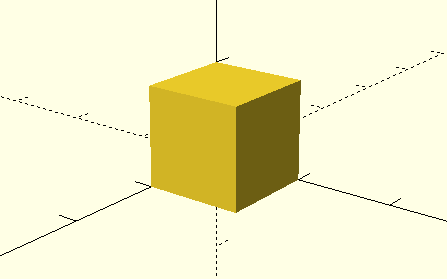
\includegraphics{Bilder/OpenSCAD_Union}
\end{Bild}
Neben solchen einfachen Objekten, wird außerdem die Möglichkeit geboten, komplexere Objekte wie Polygone (\icode{polygon()}) zu erstellen und diese dann ausgehend vom zweidimensionalen Polygon in ein dreidimensionales Polygon umzuwandeln (\icode{linear\_extrude()}), welches vor allem das Umwandeln von komplexen Formen in Objekte erleichtert. \\
Die Anweisungen, welche OpenSCAD zum Modellieren verwendet, werden in einfachen Textdateien im \q{.scad}-Format gespeichert.
Die Simplizität dieser Textdateien erlaubt es, die aus dem zu entwickelnden Programm erhaltenen Anweisungen in .scad-Dateien zu speichern, welche von OpenSCAD eingelesen, eingesehen und bearbeitet werden können. \\
%Drucken
Die Modelle, die so mit OpenSCAD erstellt wurden, können anschließend mit dem 3D-Drucker ausgedruckt werden.
Dazu werden die Modelle in Dateien des \q{.stl}-Formats konvertiert, welche schlussendlich mittels der dem 3D-Drucker beiliegenden Software entweder durch einen USB-Anschluss des 3D-Druckers oder auf einer SD-Karte gespeichert ausgedruckt werden.
Auch an dieser Stelle des Modellierungsvorganges bietet sich OpenSCAD wieder an, da dieses die Option zur Konvertierung vom .scad-Format zu .stl bietet.
\todoinline{diesen Druckteil evtl. in den Hauptteil verlagern}

\section{3D-Drucker MakerBot Replicator\texttrademark\ 2}
%Erklärung 3D-Drucker
Der vorliegende 3D-Drucker ist das Modell Replicator\texttrademark\ 2 der Firma MakerBot.
Dieser Drucker verfügt über eine höhenverstellbare Grundplatte, auf der das Filament\footnote{Filament bezeichnet das Material, welches der 3D-Drucker zum Drucken verwendet.} aufgetragen und das finale Objekt gedruckt wird, und einen sogenannten \q{Extruder}, welcher die Funktion übernimmt, das zu druckende Filament zu erhitzen und mit einer konstanten Filamentbreite auf die Grundplatte bzw. das gedruckte Objekt aufzutragen. 
Mithilfe dieser zwei Hauptbestandteile wird schichtweise Filament aufgetragen, welches aushärtet und so nach und nach das Objekt bildet. \\
Die Höhe der Grundplatte wird während des Druckvorganges automatisch vom Drucker variiert und nach Abschluss des Druckens wieder auf den Ausgangszustand zurückgesetzt.
Um die Beweglichkeit des Extruders zu garantieren, ist dieser auf drei Achsen befestigt, sodass drei Motoren ihn auf diesen Achsen verschieben können. \\
Abhängig vom Filament bzw. der Temperatur, bei der dieses aufgetragen wird, der Bewegungsgeschwindigkeit des Extruders und der Filamentstärke, die der Extruder aufträgt, lässt sich die gewünschte Druckqualität anpassen.
Eine niedrige Qualität ist dabei in den meisten Fällen mit einer erheblich kürzeren Druckzeit verbunden. \\
Die Druckzeit wird außerdem von der eingestellten Ausfüllung von geschlossenen Objekten und dem Hinzufügen von Druckhilfen beeinflusst.
So kann man Quader zum Beispiel nicht komplett mit Filament füllen lassen, sondern mit einem Bienenwabenmuster durchsetzen, sodass nur ein geringer Teil des Objektes ausgefüllt wird.
Zusätzlich zu dem eigentlichen Druckergebnis wird unter jedes gedruckte Element ein dünner Untergrund gedruckt, welcher leicht von der Grundplatte und vom gedruckten Modell zu trennen ist und so eine Beschädigung beim Entfernen des Objekts vom Drucker verhindert.
Außerdem werden bei Überhängen zusätzliche Stützen angebracht, um ein Absacken des noch nicht fest gewordenen Filaments zu verhindern. 
Indem so also ein stark verringerter Betrag an Filament aufgetragen werden muss, wird auch die Druckzeit drastisch reduziert. \\
Beim Drucken von Objekten ist neben Anpassungen zur Kontrolle der Druckqualität und Druckzeit außerdem zu beachten, dass die Grundplatte nur auf einer begrenzten Fläche bedruckbar ist.
Entsprechend dieser möglichen Maße sollten also alle Objekte in ihrer Größe angepasst werden.
% [28.5 x 15.3 x 15.5 cm]
